% !TEX root = ../build-polygon/proof-recursion.tex


\section{Polygon zkEVM \label{section:polygon:zkevm}}

\subsection{Architecture \label{subsec:zkEVM:architecture}}

In this section, we provide the concrete blocks and steps used to
prove the correct execution of a batch of transactions (or several batches)
by our zkEVM using recursion, aggregation and composition.
As previously mentioned, generating a proof has two phases. 
The first phase is a setup executed only once per STARK computation definition. 
In our case, the STARK computation is the processing of batches by our zkEVM.  
In the setup phase, the different artifacts needed to generate proofs are preprocessed.
The second phase is when actually proofs are generated for given inputs (i.e. batches of transactions).
An overview of the overall process can be observed in figure \ref{fig:architecture-aggregation-recursion-composition}.

\begin{figure}[H]
\centering
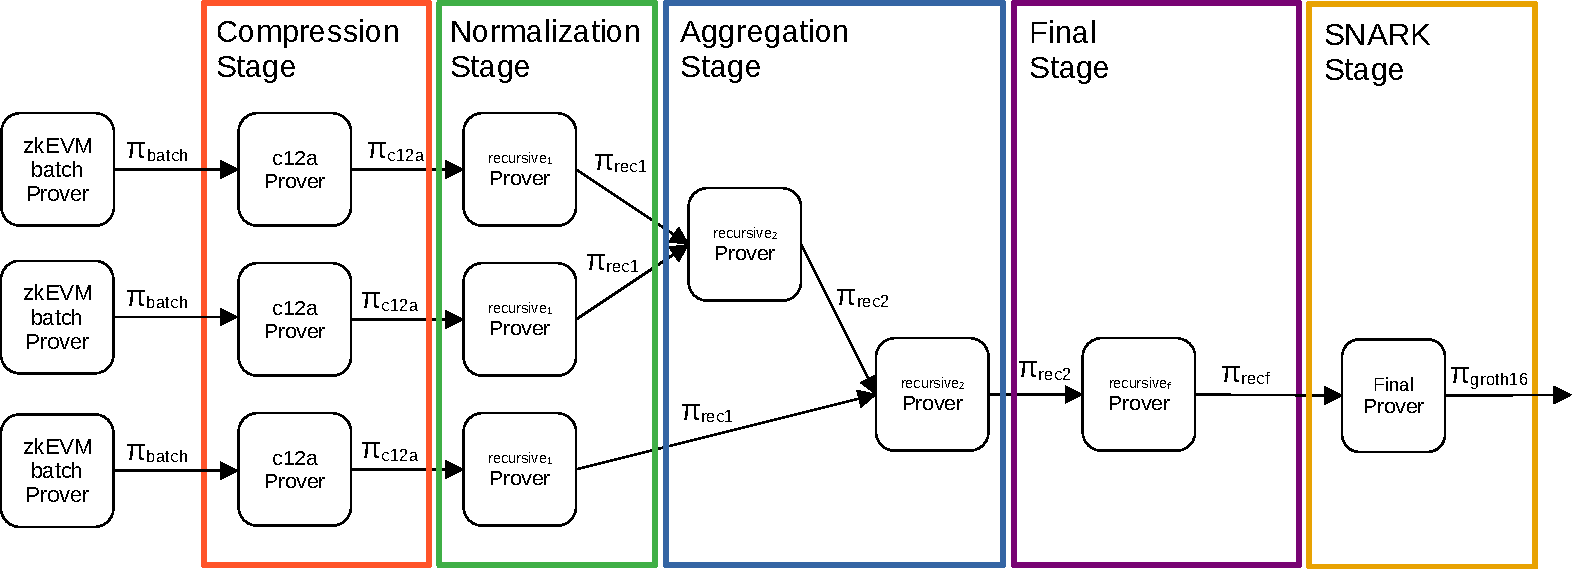
\includegraphics[width=\textwidth]{\recursiondir/figures/recursive-diagram-groth}
\caption{Proving architecture with recursion, aggregation and composition.}
\label{fig:architecture-aggregation-recursion-composition}
\end{figure}

Recall that the first STARK generates such a big proof since it has a lot of polynomials so its attached FRI uses a low blowup factor. Henceforth, a first \textit{Compression Stage} its invoked in each batch's proof, aiming to reduce the number of polynomials used, allowing to augment the blowup factor and therefore, reduce the proof size.  

Once the compression step has been completed, a proof aggregation stage will be in charge of joining several batches proofs into a single proof proving each of the single proofs all at once. The way of proceeding will be to construct a binary tree of proofs by aggregating two by two each of them. We will call this the \textit{Aggregation Stage}. 


However, since the aggregation of two proofs requires the constant root of the previous circuits through a public input coming from the previous circuit, there exists a \textit{Normalization Stage} which is in charge of transforming the obtained verifier circuit verifying the \texttt{c12a} proof into a one making the constant root public to the next circuit. This step allows each aggregator verifiers and the normalization verifiers to be exactly the same, permitting successful aggregation via a recursion. 

Once the normalization step has been finished, its time for aggregation. In this step we are going to join two batches' proofs together, which will be done many times until only one proof spares. In order to do so, a circuit capable of aggregating two verifiers is created. However, as we can see in the figure below, the inputs of this stage can be proofs of the kind $\pi_{\text{re1}}$ coming from the previous normalization stage, or  already aggregated proofs $\pi_{\text{re2}}$. This allows us to aggregate two $\pi_{\text{re1}}$ proofs, two $\pi_{\text{re2}}$ proofs or a combination of a $\pi_{\text{re1}}$ and a $\pi_{\text{re2}}$ proofs. Henceforth, this aggregation stage has to take into account this fact in its design. 


Observe that the \textit{Aggregation Stage} needs to be designed in order to accept either already aggregated proofs or only compressed ones. 
%\begin{figure}[H]
%\centering
%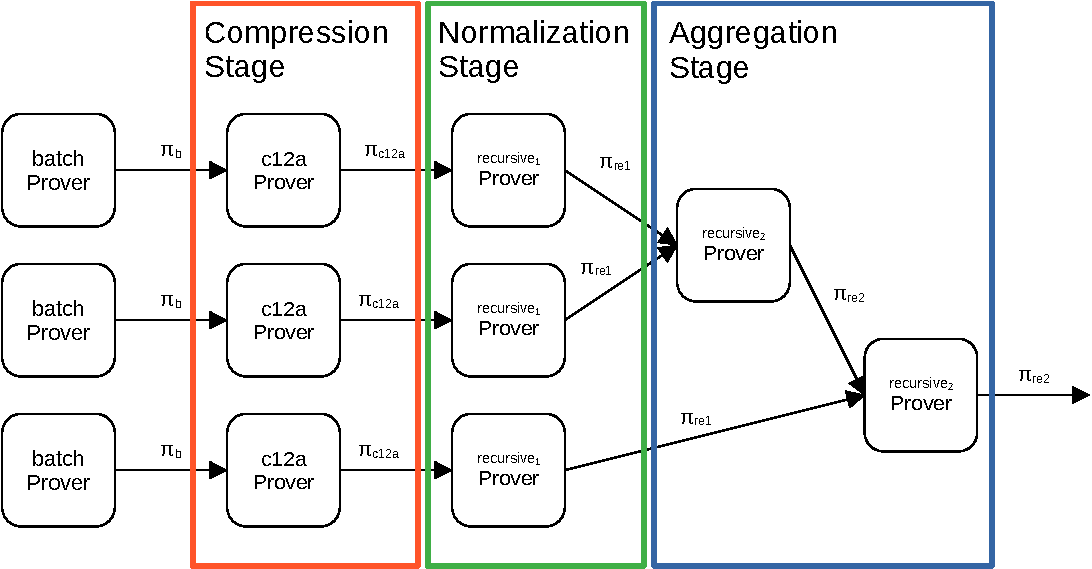
\includegraphics[width=\textwidth]{\recursiondir/figures/recursive-diagram-aggregation}
%\caption{Aggregation of proofs.}
%\label{fig:recursive-aggregation-intro}
%\end{figure}
The \textit{Final Stage} is the very last STARK step among the recursion process, which is in charge of verifying a $\pi_{\text{re2}}$ proof over a completely different finite field, the one defined by the \texttt{bn128} elliptic curve. More specifically, the hash in charge of generating the transcript will work over the field of the \texttt{bn128} curve. Hence, all the challenges (and so, all polynomials) will belong to this new field. This is done in this way because, in the next step of the process, a SNARK Groth16 proof, which works over elliptic curves, will be generated. In this step is very similar to the others, instantiating a verifier circuit for $\pi_{\text{re2}}$ but, in this case, $2$ constants roots should be provided (one for each of the proofs aggregated in the former step). 


%\begin{figure}[H]
%\centering
%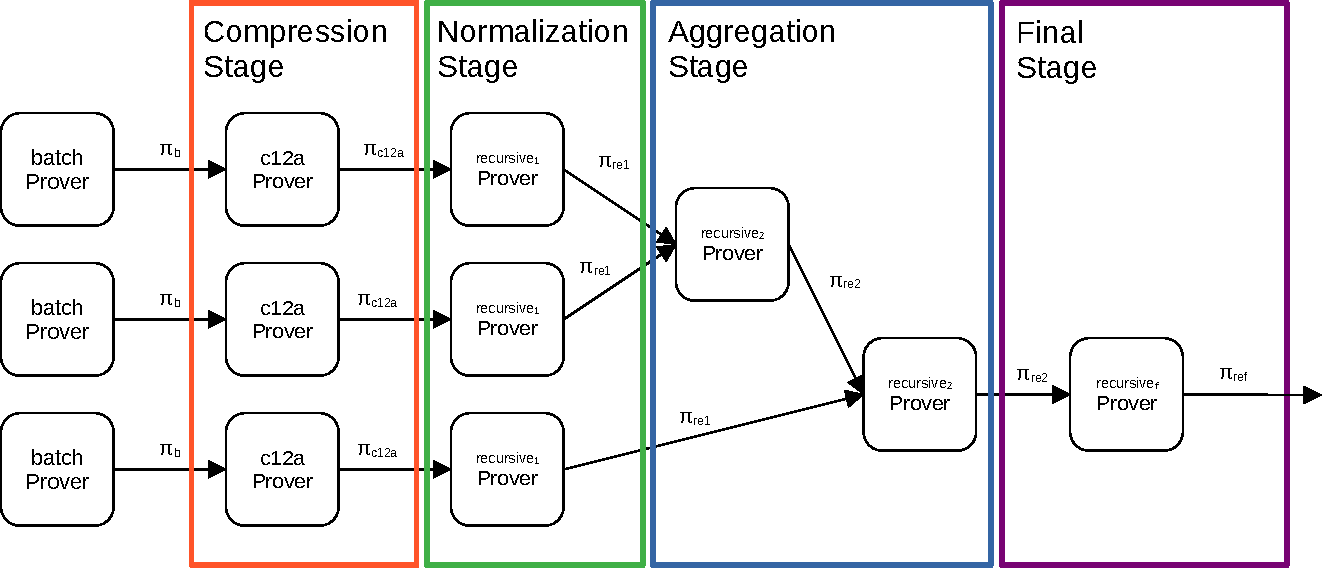
\includegraphics[width=\textwidth]{\recursiondir/figures/recursive-diagram-final}
%\caption{Final stage of the recursion.}
%\label{fig:recursivef-stage}
%\end{figure}

The last step of the whole process is called \textit{SNARK Stage}, and it purpose is to produce a Groth16 proof $\pi_{\text{groth16}}$ verifying the previous $\pi_{\text{ref}}$ proof. In fact, Groth16 can be replaced with any other SNARK proof. A SNARK is chosen here in order to reduce both verification complexity and proof size, which have constant complexity unlike STARK proofs. The $\pi_{\text{groth16}}$ proof will be sent to the verifier so that he/she can verify it. 


As a final remark, one should observe that the whole set of public inputs are being passed as inputs in each proof of the whole recursion procedure. The set of all public inputs is listed below (see the technical documents about the zkEVM L2 state management and the bridge):

\vspace{0.15cm}
\begin{compactitem}

\item \texttt{oldStateRoot}

\item \texttt{oldAccInputHash}

\item \texttt{oldBatchNum}

\item \texttt{chainId}

\item \texttt{midStateRoot}

\item \texttt{midAccInputHash}

\item \texttt{midBatchNum}

\item \texttt{newStateRoot}

\item \texttt{newAccInputHash}

\item \texttt{localExitRoot}

\item \texttt{newBatchNum}
\end{compactitem}

Next, let's describe the details of the steps and processes performed in each phase.

%%%%%%%%%%%%%%%%%%%%%%%%%%%%%%%%%%%%%%%%%%%%%%%%%%%%%%%%%
\subsection{Setup Phase}

The setup phase is a pre-processing phase in which all the artifacts for generating proofs are created. This includes the generation of intermediate circuits, which 
are a finite set of circuits that allow arbitrary combinations of proof recursions and proof aggregations.


%%%%%%%%%%%%%%%%%%%%%%%%%%%%%%%%%%%%%%%%%%%%%%%%%%%%%%%%%
\subsubsection{Build the zkEVM STARK}

As shown in Figure \ref{fig:zkevm:build}, we start by building the ROM of the zkEVM state machine, which is the program containing the instructions for the the executor that will generate the execution trace of the zkEVM. We also build the PIL that validates the execution trace. The ROM will, in fact, generate all the constant values for the execution trace of the zkEVM. Observe that, as said before, committed polynomials are not needed in the setup phase, so we need not run the executor of the zkEVM in order to generate them at this point. 

%TODO mirar que parte del starkInfo hace falta para generar el circom.

\begin{figure}[H]
\centering
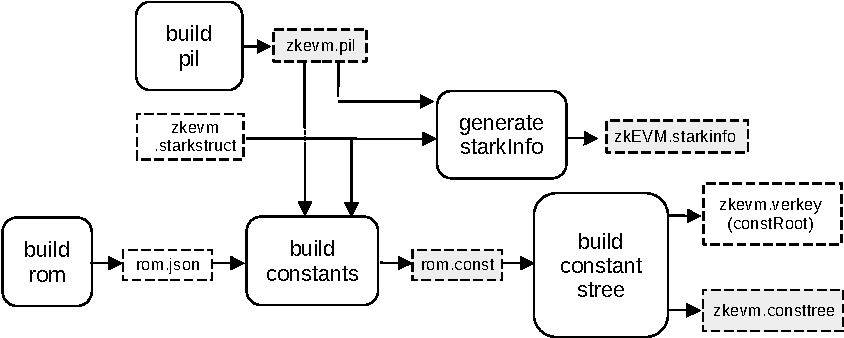
\includegraphics[width=0.85\textwidth]{\recursiondir/figures/zkevm-build}
\caption{Build the zkEVM STARK}
\label{fig:zkevm:build}
\end{figure}

The Merkle root of the tree of constant polynomials' evaluations, which is a hash that serves as cryptographic summary to capture all the fixed parameters of the computation, is stored as a parameter in a file called \texttt{zkevm.verkey}.
The last piece of data that is generated before building the STARK is the \texttt{starkInfo} that is necessary for automatically generating the circuit that will verify the zkEVM STARK. 
In this case, we use a blowup factor of $2$ and $128$ queries to generate the proof. 
The artifacts marked in gray will be used when generating the proof (proof generation is described in more detail in Section \ref{subsec:proof:gen:phase}). 





%%%%%%%%%%%%%%%%%%%%%%%%%%%%%%%%%%%%%%%%%%%%%%%%%%%%%%%%%
\subsubsection{Setup \stoc for the zkEVM STARK}

The next step in the setup is to generate the circuit to verify the zkEVM STARK (see Figure \ref{fig:zkevm:s2c}). 

\begin{figure}[H]
\centering
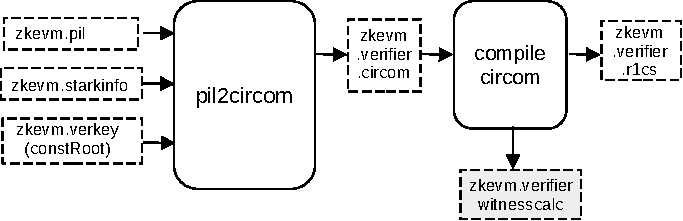
\includegraphics[width=0.8\textwidth]{\recursiondir/figures/zkevm-s2c}
\caption{Converting the zkEVM STARK verification into a circuit.}
\label{fig:zkevm:s2c}
\end{figure}


The \texttt{pil2circom} process fills an \texttt{EJS} template called \texttt{stark\_verifier.circom.ejs} with all the necessary information needed to validate the zkEVM STARK. Henceforth, we need to add the \texttt{zkevm.pil} in order to capture polynomial names, the \texttt{zkevm.starkinfo} file which specifies the blowup factor, the number of queries and the steps of the FRI-verification procedure and the \texttt{constRoot} in the \texttt{zkevm.verkey} file to automatically generates a circuit in Circom. The output Circom file \texttt{zkevm.verifier.circom} is then compiled into R1CS constraint system written in a file called \texttt{zkevm.verifier.r1cs}. This constraints will be used in the next step to generate the PIL and the constant polynomials for the next proof. 

On the other hand, the Circom compilation also outputs a witness calculator program that we call \texttt{zkevm.verifier.witnesscalc}. As it can be observed in the picture, the witness calculator program is marked in gray because it is going to be used when generating the proof.

Since our aim at the next proof generation will be compression (that is, proof size reduction) we will use a blowup factor of $4$ in this step, with $64$ queries. This information is contained in the \texttt{c12a.starkstruct} file located in the \texttt{proverjs} repository.



%%%%%%%%%%%%%%%%%%%%%%%%%%%%%%%%%%%%%%%%%%%%%%%%%%%%%%%%%
\subsubsection{Setup \ctos \texttt{c12a}}

The circuit that verifies the zkEVM STARK is called \texttt{zkevm.verifier} (or also \texttt{c12a}). This is because the PIL that is going to verify the \texttt{c12a} circuit is a \plonk{ish} circuit with custom gates and 12 polynomials aiming at compression. 

\begin{figure}[H]
\centering
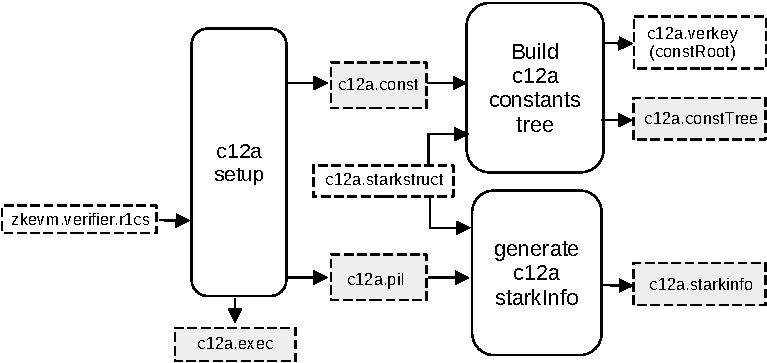
\includegraphics[width=0.85\textwidth]{\recursiondir/figures/c12a-c2s}
\caption{Convert the zkEVM verifier circuit to a STARK called \texttt{c12a}.}
\label{fig:zkevm-verifier-c2s}
\end{figure}

From the previous R1CS description of the verification circuit we are going to obtain a machine-like construction whose correct execution, which will be described by a PIL file, will be equivalent to the validity of the previous circuit. This process is started through a service called \texttt{compressor12\_setup}, where the corresponding PIL file for verifying the trace is output, as well as a binary for all the constant polynomials \texttt{c12a.const} defined by it. Moreover, a helper file called \texttt{c12a.exec} is generated by the same service. This helper file will contain all the necessary rules that will allow us to shuffle all the witness values, which will be computed later on, into the corresponding position of the execution trace. The design of this shuffling, together with the the connections defined in the constants polynomials \texttt{c12a.const} will ensure that, for a honest prover, this newly generated trace is valid whenever the previous circuit is. 

In order to finish the set up phase, having all the FRI-related parameters willing to be used in this step stored in a \texttt{c12a.starkstruct} file (located in the prover repository), we can generate the \texttt{c12a.starkinfo} file through the \texttt{generate\_starkinfo} service and build the constants' tree (and its respectively constant root). 




\subsubsection{Setup \stoc for \texttt{recursive1}}

Up to this point we have a STARK proof $\pi_{\text{c12a}}$ verifying the first big STARK proof $\pi$. The idea now is, as before, generate a Circom circuit that verifies $\pi_{\text{c12a}}$ by miming the FRI verification procedure. To do that, we generate a verifier circuit \texttt{c12a.verifier.circom} from the previously obtained \texttt{c12a.pil} file, the \texttt{c12a.starkinfo} file and the constant root \texttt{c12a.verkey.constRoot} by filling the \texttt{stark\_verifier.circom.ejs} template as before.

In this case, in seek of normalization, we need to briefly modify this circuit in order to include the constant root as a public input. Observe that, since we are not still aggregating, the constant root will not be actually used here, though this will be extremely important in the aggregation stage, where all the constants for the computation, which depend on the previous circuit, need to be provided as public inputs. This is done by using \texttt{recursive1.circom} file and importing inside the previously generated \texttt{c12a.verifier.circom} circuit as a library. The verifier circuit is instantiated inside \texttt{recursive1.circom}, connecting all the necessary wires and including the constant root to the set of publics. 

The output circom file \texttt{recursive1.circom} it is compiled into a R1CS \texttt{recursive1.r1cs} file and a witness calculator program \texttt{recursive1.witnesscal} which will be both used later on in order to build and fill the next execution trace. 

\begin{figure}[H]
\centering
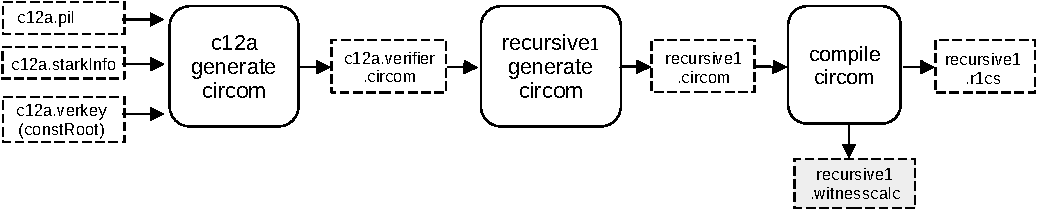
\includegraphics[width=\textwidth]{\recursiondir/figures/c12a-s2c}
\caption{Convert the c12a STARK to a c12a verifier circuit.}
\label{fig:c12a-s2c}
\end{figure}

\subsubsection{Setup \ctos for \texttt{recursive1}}

As before, from the previous R1CS description of the verification circuit we are going to obtain a machine-like construction whose correct execution, which will be described by a PIL \texttt{recursive1.pil} file, will be equivalent to the validity of the previous circuit. Also, a binary for all the constant polynomials \texttt{recursive1.const} defined by it and the helper file providing the witness values allocation into its corresponding position of the execution trace \texttt{recursive1.exec} are generated.

In order to finish the set up phase, having all the FRI-related parameters willing to be used in this step stored in a \texttt{recursive.starkstruct} file (located in the prover repository), we can generate the \texttt{recursive1.starkinfo} file through the \texttt{generate\_starkinfo} service and build the constants' tree (and its respectively constant root). In this case, we are using a blowup factor of $2^4 = 16$, allowing the number of queries to be $32$. 

\begin{figure}[H]
\centering
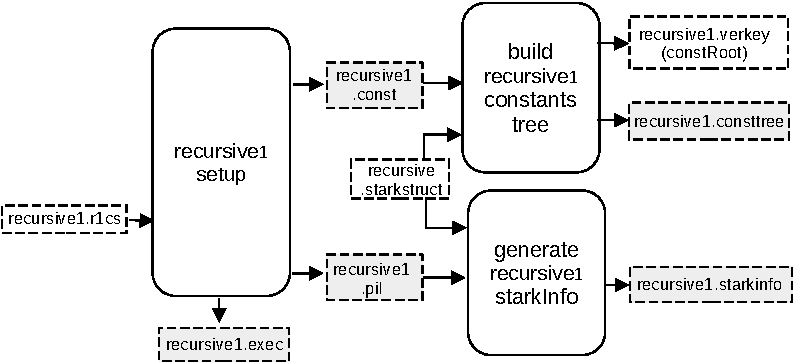
\includegraphics[width=.85\textwidth]{\recursiondir/figures/recursive1-c2s}
\caption{Convert the \texttt{recursive1} circuit to its associated STARK.}
\label{fig:recursive1-c2s}
\end{figure}



\subsubsection{Setup \stoc for \texttt{recursive2}}

Up to this point we have a STARK proof $\pi_{\text{re1}}$ verifying the proof $\pi_{\text{c12a}}$. As before, we generate a Circom circuit that verifies $\pi_{\text{re1}}$ by miming the FRI verification procedure. To do that, we generate a verifier circuit \texttt{recursive1.verifier.circom} from the previously obtained \texttt{recursive1.pil} file, the \texttt{recursive1.starkinfo} file and the constant root \texttt{recursive1.verkey.constRoot} by filling the verifier \texttt{stark\_verifier.circom.ejs} template.

After the verifier is generated using the template, we will also use a template to create another Circom that aggregates two verifiers. Note that, in the previous step, the constant root is passed harcoded into the circuit from an external file. But this was intended as a normalization, allowing the previous circuit and each ones verifying each of both proofs to have exactly the same form, allowing recursion being possible. Henceforth, this \texttt{recursive2.circom} circuit has two verifiers and a two multiplexors that are actually deciding the form of each of the verifiers: if the proof has $\pi_{\text{re1}}$ form, the hardcoded constant root is input but, if the proof has $\pi_{\text{re2}}$ form, the constant root should be connected as input signal, coming from a previous circuit. 

A schema of the \texttt{recursive2} circuit generated is as shown in Figure \ref{fig:recursive2-circuit}. Observe that, since the upper proof has the $\pi_{\text{re2}}$ form, the Multiplexor does not provides the constant root \texttt{rootC} to the Verifier A to hardcode it because this verifier should get it trough a public input from the previous circuit. Otherwise, the lower proof has the $\pi_{\text{re1}}$ form, so the Multiplexor let is pass trough the constant root into the Verifier B so that it can be hardcoded it when the corresponding template is filled. 

\begin{figure}[H]
	\centering
	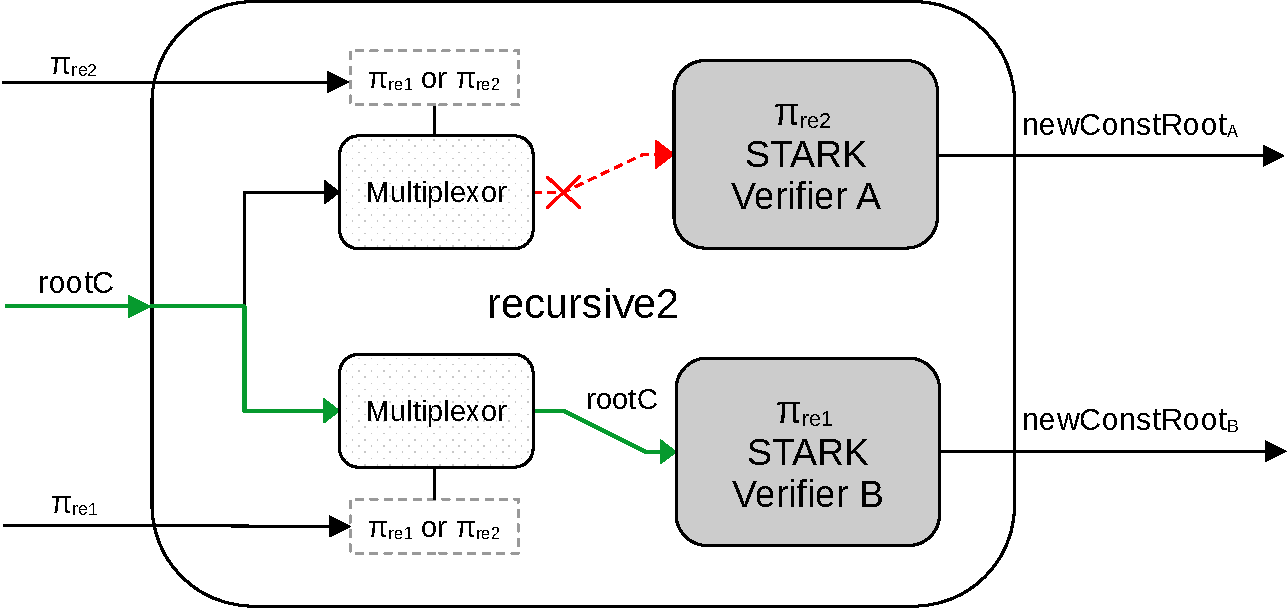
\includegraphics[width=0.9\textwidth]{\recursiondir/figures/recursive2-circuit}
	\caption{\texttt{recursive2} circuit.}
	\label{fig:recursive2-circuit}
\end{figure}


The output circom file \texttt{recursive2.circom}, obtained running a different script called \texttt{genrecursive} it is compiled into a R1CS \texttt{recursive2.r1cs} file and a witness calculator program \texttt{recursive2.witnesscal} which will be both used later on in order to build and fill the next execution trace. 

\begin{figure}[H]
\centering
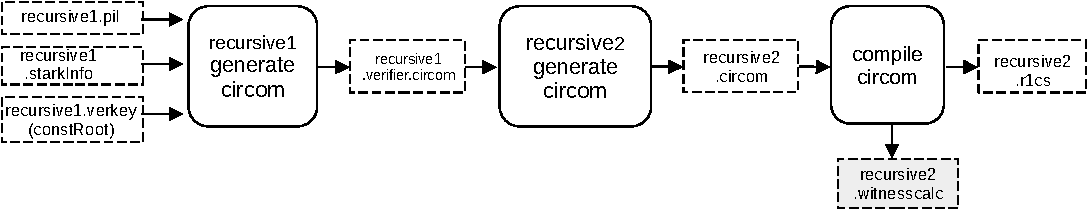
\includegraphics[width=\textwidth]{\recursiondir/figures/recursive1-s2c}
\caption{Convert the \texttt{recursive1} STARK to its verifier circuit called \texttt{recursive2}.}
\label{fig:recursive1-s2c}
\end{figure}




\subsubsection{Setup \ctos for \texttt{recursive2}}

As before, from the previous R1CS description of the verification circuit we are going to obtain a machine-like construction whose correct execution, which will be described by a PIL \texttt{recursive2.pil} file, will be equivalent to the validity of the previous circuit. Also, a binary for all the constant polynomials \texttt{recursive2.const} defined by it and the helper file providing the witness values allocation into its corresponding position of the execution trace \texttt{recursive2.exec} are generated.

In order to finish the set up phase, having all the FRI-related parameters willing to be used in this step stored in a \texttt{recursive.starkstruct} file (located in the prover repository), we can generate the \texttt{recursive2.starkinfo} file through the \texttt{generate\_starkinfo} service and build the constants' tree (and its respectively constant root). Since we want both verifiers to be exactly the same as in the previous step, we are using the same blowup factor of $2^4 = 16$, allowing the number of queries to be $32$. 

\begin{figure}[H]
	\centering
	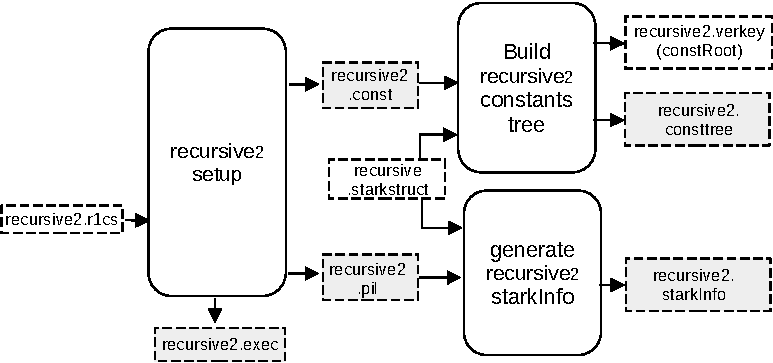
\includegraphics[width=.8\textwidth]{\recursiondir/figures/recursive2-c2s}
	\caption{Convert the \texttt{recursive2} circuit to its associated STARK.}
	\label{fig:recursive2-c2s}
\end{figure}



\subsubsection{Setup \stoc for \texttt{recursivef}}

Up to this point we have a STARK proof $\pi_{\text{re2}}$ verifying another  $\pi_{\text{re2}}$ proof (or $\pi_{\text{re1}}$ in some edge cases). The idea now is, as before, generate a Circom circuit that verifies $\pi_{\text{re2}}$ (or $\pi_{\text{re1}}$ if no aggregation is taking place) by miming the FRI verification procedure as done before. To do that, we generate a verifier circuit \texttt{recursive2.verifier.circom} from the previously obtained \texttt{recursive2.pil} file, the \texttt{recursive2.starkinfo} file and the constant roots of the previous two proofs \texttt{recursive2\_a.verkey.constRoot} and \texttt{recursive2\_b.verkey.constRoot} by filling the \texttt{stark\_verifier.circom.ejs} template as before.

The output circom file \texttt{recursivef.circom}, obtained running a different script called \texttt{genrecursivef} it is compiled into a R1CS \texttt{recursivef.r1cs} file and a witness calculator program \texttt{recursivef.witnesscal} which will be both used later on in order to build and fill the next execution trace. 

\begin{figure}[H]
\centering
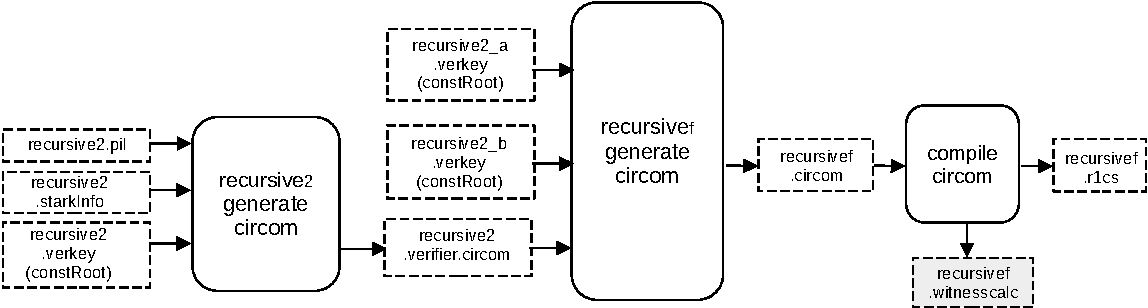
\includegraphics[width=\textwidth]{\recursiondir/figures/recursive2-s2c}
\caption{Convert the \texttt{recursive2} STARK to its verifier circuit called \texttt{recursivef}.}
\label{fig:recursive2-s2c}
\end{figure}

\subsubsection{Setup \ctos for \texttt{recursivef}}

As before, from the R1CS description of the verification circuit we are going to obtain a machine-like construction whose correct execution, which will be described by a \texttt{recursive2.pil} PIL file, will be equivalent to the validity of the previous circuit. Also, a binary for all the constant polynomials \texttt{recursive2.const} defined by it and the helper file providing the witness values allocation into its corresponding position of the execution trace \texttt{recursive2.exec} are generated.

In order to finish the set up phase, having all the FRI-related parameters willing to be used in this step stored in a \texttt{recursivef.starkstruct} file (located in the prover repository), we can generate the \texttt{recursivef.starkinfo} file through the \texttt{generate\_starkinfo} service and build the constants' tree (and its respectively constant root). 

\begin{figure}[H]
\centering
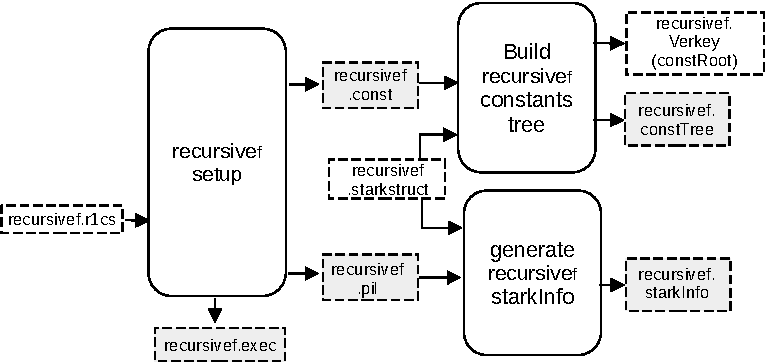
\includegraphics[width=0.8\textwidth]{\recursiondir/figures/recursivef-c2s}
\caption{Convert the recursivef circuit to its associated STARK.}
\label{fig:recursivef-c2s}
\end{figure}




\subsubsection{Setup \stoc for \texttt{final}}

Up to this point we have a STARK proof $\pi_{\text{ref}}$ verifying a proof $\pi_{\text{re2}}$. As before, we generate a Circom circuit that verifies $\pi_{\text{ref}}$ by miming the FRI verification procedure. To do that, we generate a verifier circuit \texttt{recursivef.verifier.circom} from the previously obtained \texttt{recursivef.pil} file, the \texttt{recursivef.starkinfo} file and the constant root \texttt{recursivef.verkey.constRoot} by filling the \texttt{stark\_verifier.circom.ejs} verifier template. This verifier Circom file will be imported by the \texttt{final.circom} circuit in order to generate the circuit that will be proven using Groth16 procedure. 



\begin{figure}[H]
	\centering
	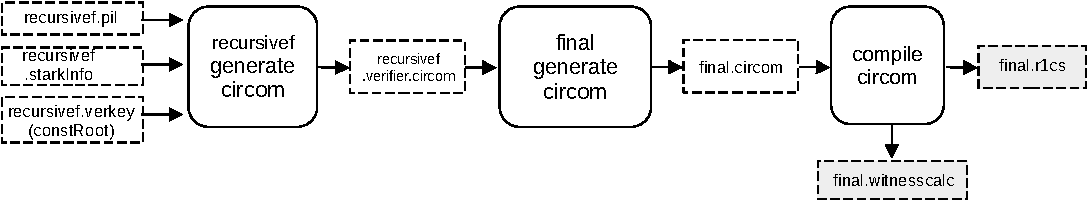
\includegraphics[width=\textwidth]{\recursiondir/figures/final-s2c}
	\caption{Convert the \texttt{recursivef} STARK to its verifier circuit that is called \texttt{final.circom}.}
	\label{fig:final-s2c}
\end{figure}



\subsection{Proof Generation Phase \label{subsec:proof:gen:phase}}

\subsubsection{Proof of the zkEVM STARK}

Up to this point we built an execution trace together with a PIL file describing the ROM of the zkEVM. Having both we can generate a STARK proof stating the correct execution of the zkEVM using the \texttt{pil-stark} tooling explained in section \ref{subsec:non_recursive_STARK}. In this step, a blowup factor of $2$ is used, so the proof having a huge amount of polynomials becomes quite big. To amend that, the next step \texttt{c12a} will be a compression step, raising the blowup factor and aiming to reduce the number of polynomials. 

\begin{figure}[H]
\centering
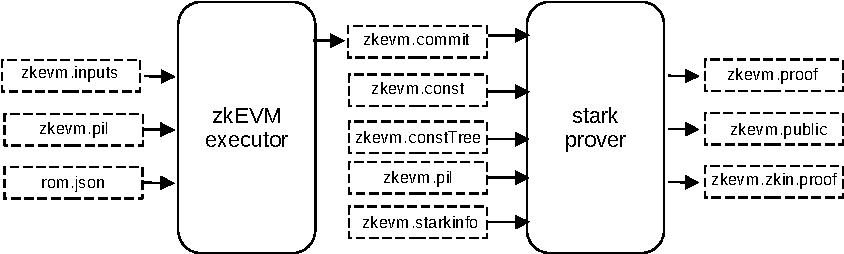
\includegraphics[width=0.85\textwidth]{\recursiondir/figures/zkevm-proof}
\caption{Generation for a zkEVM Proof}
\label{fig:recursive-zkemv-proof}
\end{figure}

To generate the proof, \texttt{main\_prover} service is used. The service requires to provide the execution trace (that is, the committed and constant polynomials files generated by the executor using the \texttt{pilcom} package), the constant tree binary file in order to be hashed to construct the constant root, the PIL file of the zkEVM ROM \texttt{zkev.pil} and all the information provided by the \texttt{zkevm.starkinfo.json} file, including all the FRI-related parameters such as the blowup factor or the configuration of the steps. 

This step differs from the next ones as it is the first and it is intended to start the recursion. However, aiming uniformization code-wise,  the Main Prover procedure choose to abstract the notion of proving and is intended to be the same at each step among the recursion. 



\subsubsection{Proof of \texttt{c12a}}


%TODO: Jose: The publics of c12a are the same as zkevm right?

To generate the proof verifying the previous \texttt{zkevm.proof}, we generate all the witness values and map them correctly into its corresponding position of the execution trace exactly in the same way as before, obtaining a binary file \texttt{ca12.commit} for the committed polynomials of the execution trace. 

Having the execution trace (that is, the committed and constant polynomials filled) and the PIL, we can generate a proof validating the previous big STARK proof. We use the same service \texttt{main\_prover} as before to do it, providing also the previously built constant tree \texttt{ca12.constTree} and the \texttt{ca12.starkinfo} file. This will generate the proof and the publics joined in the \texttt{c12a.zkin.proof} file.  

\begin{figure}[H]
\centering
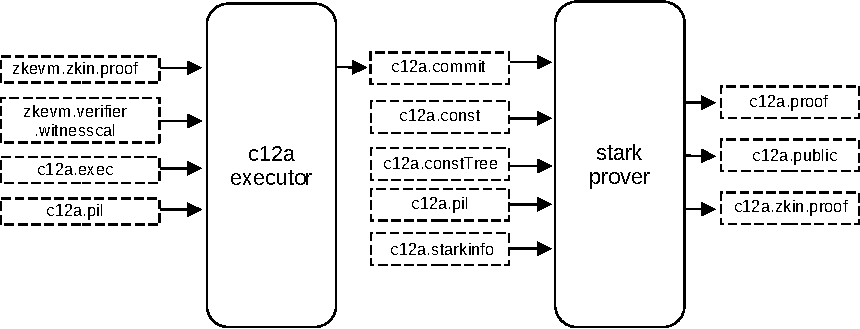
\includegraphics[width=0.77\textwidth]{\recursiondir/figures/c12a-proof}
\caption{Generate a STARK proof for \texttt{c12a}.}
\label{fig:c12a-proof}
\end{figure}



\subsubsection{Proof of \texttt{recursive1}}

To generate the proof verifying the previous \texttt{c12a.proof}, we generate all the witness values and map them correctly into its corresponding position of the execution trace exactly in the same way as before, obtaining a binary file \texttt{recursive1.commit} for the committed polynomials of the execution trace. 

Having the execution trace (that is, the committed and constant polynomials filled) and the PIL, we can generate a proof validating the previous big STARK proof. We use the same service \texttt{main\_prover} as before to do it, providing also the previously built constant tree \texttt{recursive1.constTree} and the \texttt{recursive1.starkinfo} file. This will generate the proof and the publics joined in the \texttt{recursive1.zkin.proof} file. 

\begin{figure}[H]
\centering
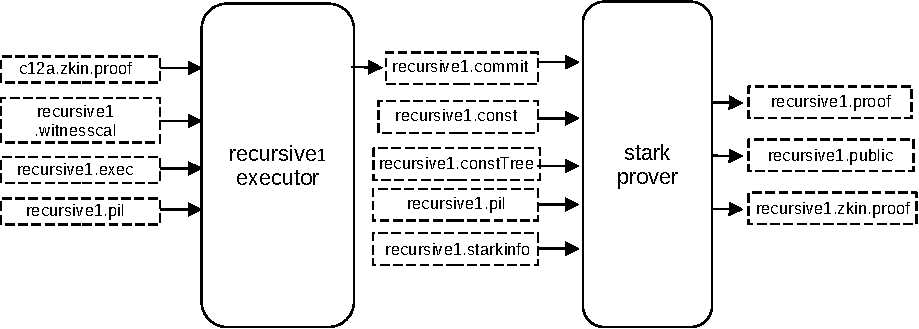
\includegraphics[width=0.85\textwidth]{\recursiondir/figures/recursive1-proof}
\caption{Generate a STARK proof for \texttt{recursive1}.}
\label{fig:recursive1-proof}
\end{figure}



\subsubsection{Proof of \texttt{recursive2}}

To generate the proof verifying the previous \texttt{recursive1.proof}, we generate all the witness values and map them correctly into its corresponding position of the execution trace exactly in the same way as before, obtaining a binary file \texttt{recursive2.commit} for the committed polynomials of the execution trace. 

Having the execution trace (that is, the committed and constant polynomials filled) and the PIL, we can generate a proof validating the previous big STARK proof. We use the same service \texttt{main\_prover} as before to do it, providing also the previously built constant tree \texttt{recursive2.constTree} and the \texttt{recursive2.starkinfo} file. This will generate the proof and the publics joined in the \texttt{recursive2.zkin.proof} file. 

\begin{figure}[H]
\centering
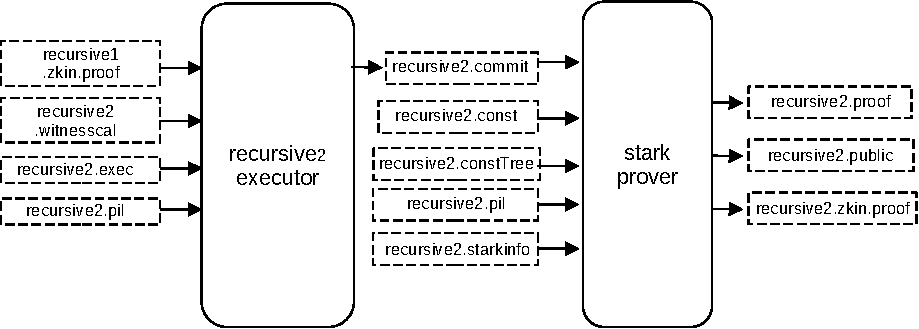
\includegraphics[width=\textwidth]{\recursiondir/figures/recursive2-proof}
\caption{Generate a STARK proof for \texttt{recursive2}.}
\label{fig:recursive2-proof}
\end{figure}


\subsubsection{Proof of \texttt{recursivef}}

To generate the proof verifying the previous \texttt{recursive2.proof}, we generate all the witness values and map them correctly into its corresponding position of the execution trace exactly in the same way as before, obtaining a binary file \texttt{recursivef.commit} for the committed polynomials of the execution trace. 

Having the execution trace (that is, the committed and constant polynomials filled) and the PIL, we can generate a proof validating the previous big STARK proof. We use the same service \texttt{main\_prover} as before to do it, providing also the previously built constant tree \texttt{recursivef.constTree} and the \texttt{recursivef.starkinfo} file. This will generate the proof and the publics joined in the \texttt{recursivef.zkin.proof} file. 


\begin{figure}[H]
\centering
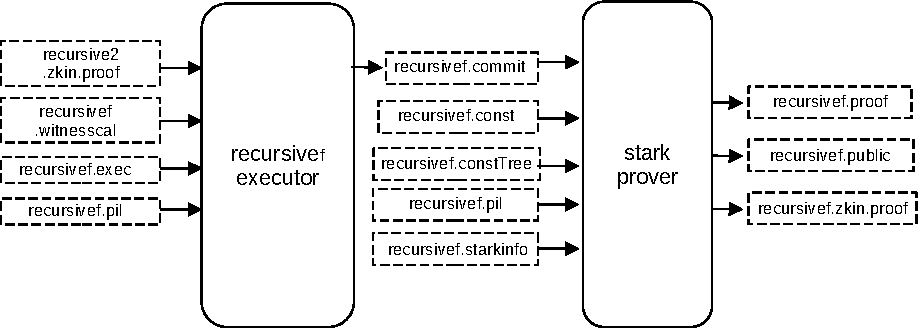
\includegraphics[width=0.77\textwidth]{\recursiondir/figures/recursivef-proof}
\caption{Generate a STARK proof for \texttt{recursivef}.}
\label{fig:recursivef-proof}
\end{figure}



\subsubsection{Proof of \texttt{final}}

The last circuit, \texttt{final.circom} is the one used to generate the proof.
At this moment a Groth16 proof is generated.
